\localauthor{Thomas Kirz}

Zusätzlich zu den Tests aus dem Pflichtenheft wurden folgende Tests geschrieben,
um verschiedene Sicherheitsaspekte des Systems zu testen.
Es handelt sich auch hier um Integrationstests, die das Selenium-Framework verwenden.

Diese Tests liefen durch, nach Korrektur von Fehlern, die in Kapitel ???? beschrieben wurden und nichts mit hier zu testenden Sicherheit zu tun hatten.
Nur der Name des Session-Cookies bzw.~URL-Parameters wurde wie in der Feinspezifikation vorgegeben von \code{jsessionid} zu \code{sessionid} geändert, da diese Einstellung in der web.xml-Datei noch gefehlt hatte.

Die geprüften Bedingungen für den Erfolg der Tests sind \textbf{fett} geschrieben.

\subsection{Injection}\label{subsec:injection-test}
Dieser Test prüft den Schutz gegen SQL- und HTML/JavaScript-Injection.

Dazu wird ein Nutzerkonto angelegt mit dem Titel \emph{";DROP table user;} (auch bekannt als Little Bobby Tables, siehe Abbildung~\ref{fig:xkcd}).
Wäre hier SQL-Injection möglich, könnte dieser Titel bei Ausführung des \code{INSERT}-Statements in der Datenbank
die \code{user}-Tabelle löschen.
\textbf{Es wird geprüft, dass die Nutzerdaten auf der Profilseite korrekt angezeigt werden.}

\begin{figure}[h]
    \centering
    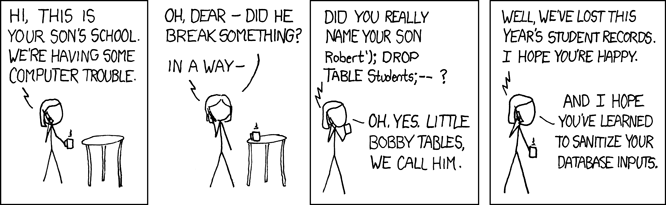
\includegraphics[width=0.8\textwidth]{graphics/xkcd}
    \caption[XKCD]{\emph{Exploits of a Mom}\footnotemark}
    \label{fig:xkcd}
\end{figure}
\footnotetext{Abbildung von \href{https://xkcd.com/327/}{XKCD}, lizenziert unter \href{https://creativecommons.org/licenses/by-nc/2.5/legalcode}{Namensnennung-Nicht kommerziell 2.5 Generic (CC BY-NC 2.5)}}

Dann lädt der Nutzer eine Einreichung mit dem Titel \emph{<script>alert('XSS');</script>} hoch.
\textbf{Der Titel soll jetzt so wie eingegeben angezeigt werden anstatt dass der JavaScript-Code ausgeführt wird.}

\subsection{Aufruf ohne Login}\label{subsec:unauthorized-test}
Ohne sich anzumelden, wird versucht, die Startseite (für authorisierte Nutzende) aufzurufen.
\textbf{Der Nutzer soll auf die Anmeldeseite weitergeleitet werden.}

\subsection{Session Fixation}\label{subsec:session-fixation-test}
Für diesen Test werden Cookies deaktiviert, damit die Session-ID in die URL geschrieben wird.

Ein Nutzer ruft die Webseite auf und bekommt eine Session-ID\@.
Mit dieser Session meldet er sich an.
\textbf{Wird die Webseite nun erneut mit der alten Session-ID aufgerufen, darf der Nutzer nicht angemeldet sein.}

\subsection{Insecure Direct Object Reference}\label{subsec:idor-test}
Dieser Test prüft, dass ein Nutzer nicht unberechtigt auf Inhalte zugreifen kann, indem er deren ID herausfindet.

Dazu legt ein angemeldeter Nutzer eine Einreichung an.
Ein weiterer, neu registrierter Nutzer versucht jetzt,
die Seite für diese Einreichung (mit richtiger ID als URL-Parameter) aufzurufen.
\textbf{Die Einreichung darf nicht angezeigt werden; der Nutzer wird auf eine 404-Seite weitergeleitet.}
